\documentclass[11pt,a4paper]{article}
\usepackage[margin=25mm]{geometry}
\usepackage[T1]{fontenc}
\usepackage{lmodern,pdfpages}
\usepackage[hidelinks]{hyperref}
\begin{document}
\section*{Complete incoming sidebar mathematics}
Complete author-generated working texts follow in separate parts. Their original claims, qualifications, citations and proofs are preserved. Mirroring is not mathematical validation.
\tableofcontents
\bigskip
\noindent\textbf{Exact fluid constructions and the Navier--Stokes question}\par
\noindent Complete source: \path{sidebar/fluid/tex/main.tex}.\par\medskip
\noindent\textbf{Heat transport on the retained inverse-fibre cover}\par
\noindent Complete source: \path{sidebar/heat/tex/main.tex}.\par\medskip
\noindent\textbf{Arithmetic trace quotient and exact heat transport}\par
\noindent Complete source: \path{sidebar/connes/tex/main.tex}.\par\medskip
\noindent\textbf{Retained fibres, nonstandard Riemann hypotheses, and geometric complexity}\par
\noindent Complete source: \path{sidebar/gct/tex/main.tex}.\par\medskip
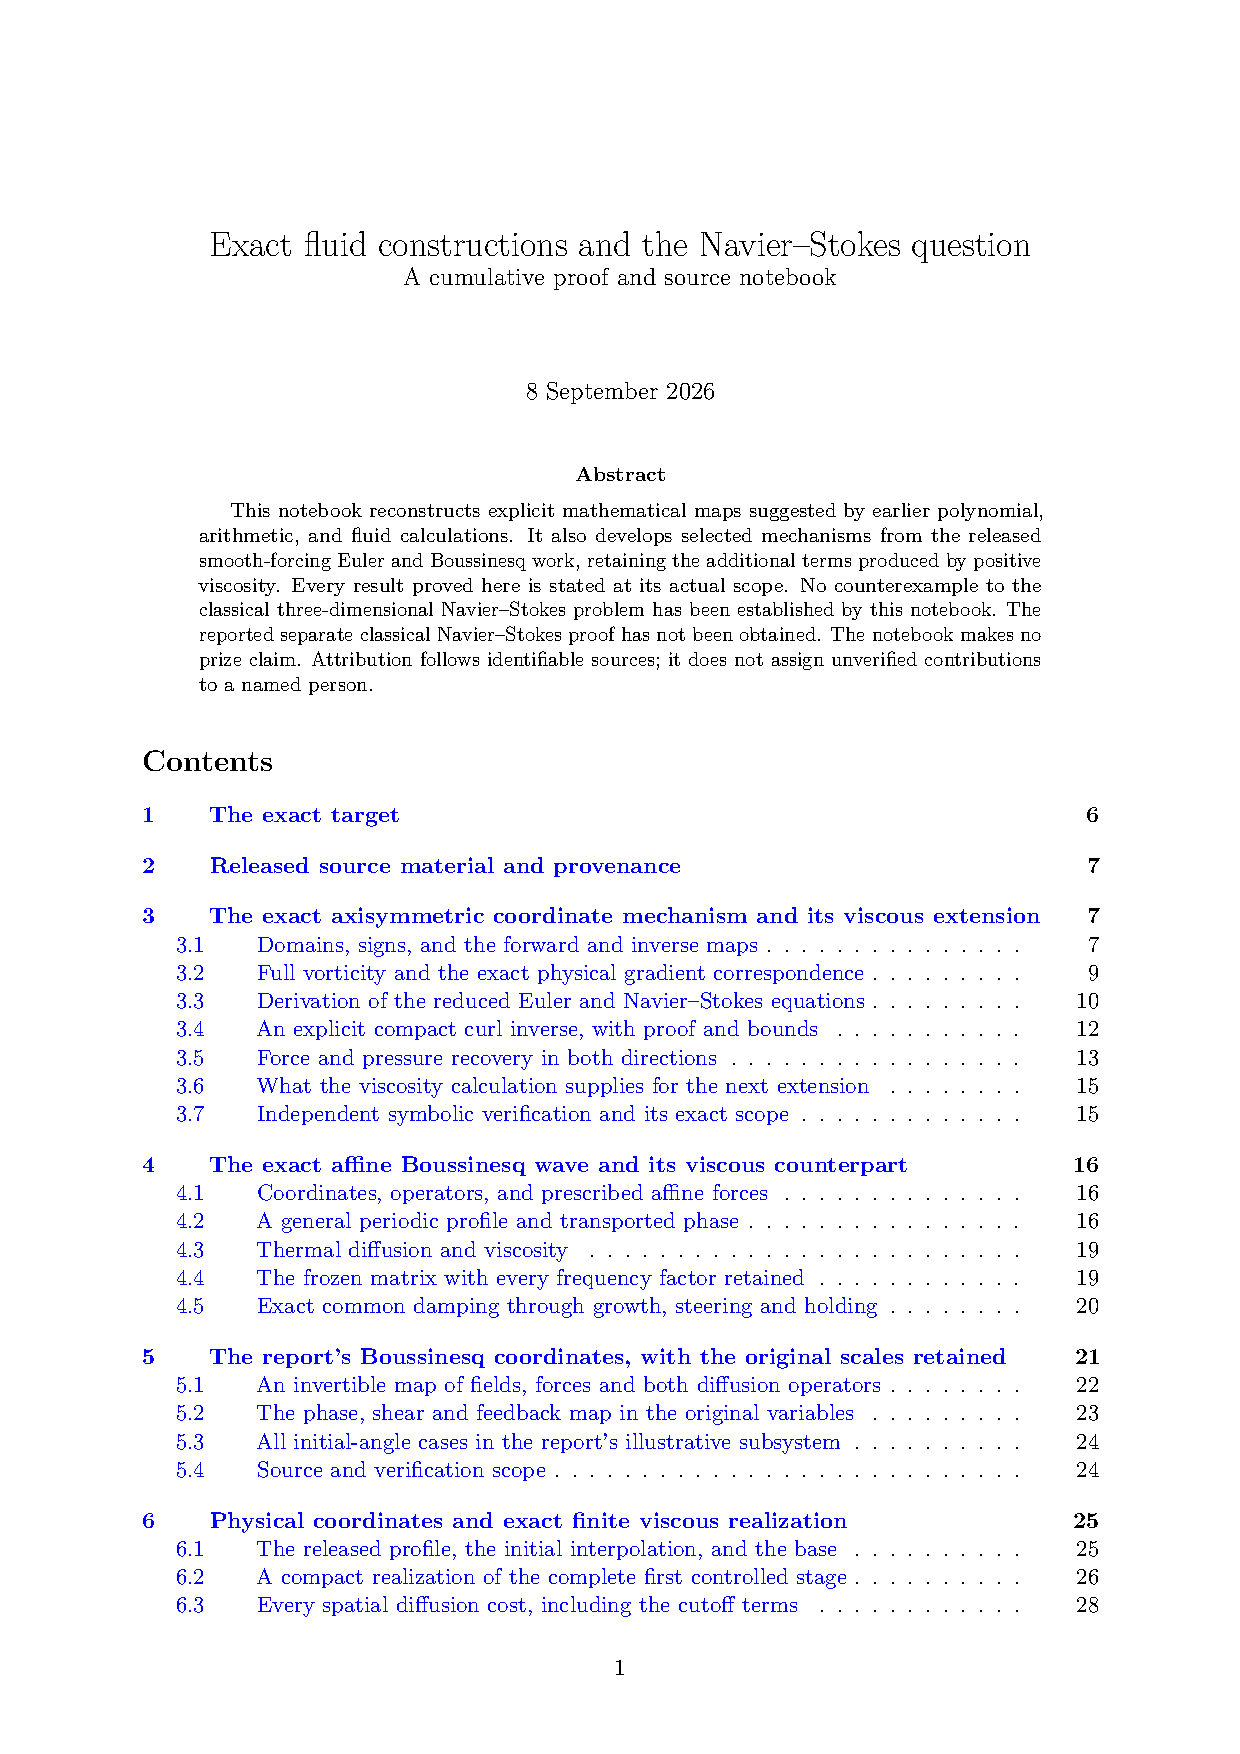
\includepdf[pages=-,addtotoc={1,section,1,{Exact fluid constructions and the Navier--Stokes question},sidebar-fluid}]{sidebar/fluid/reader.pdf}
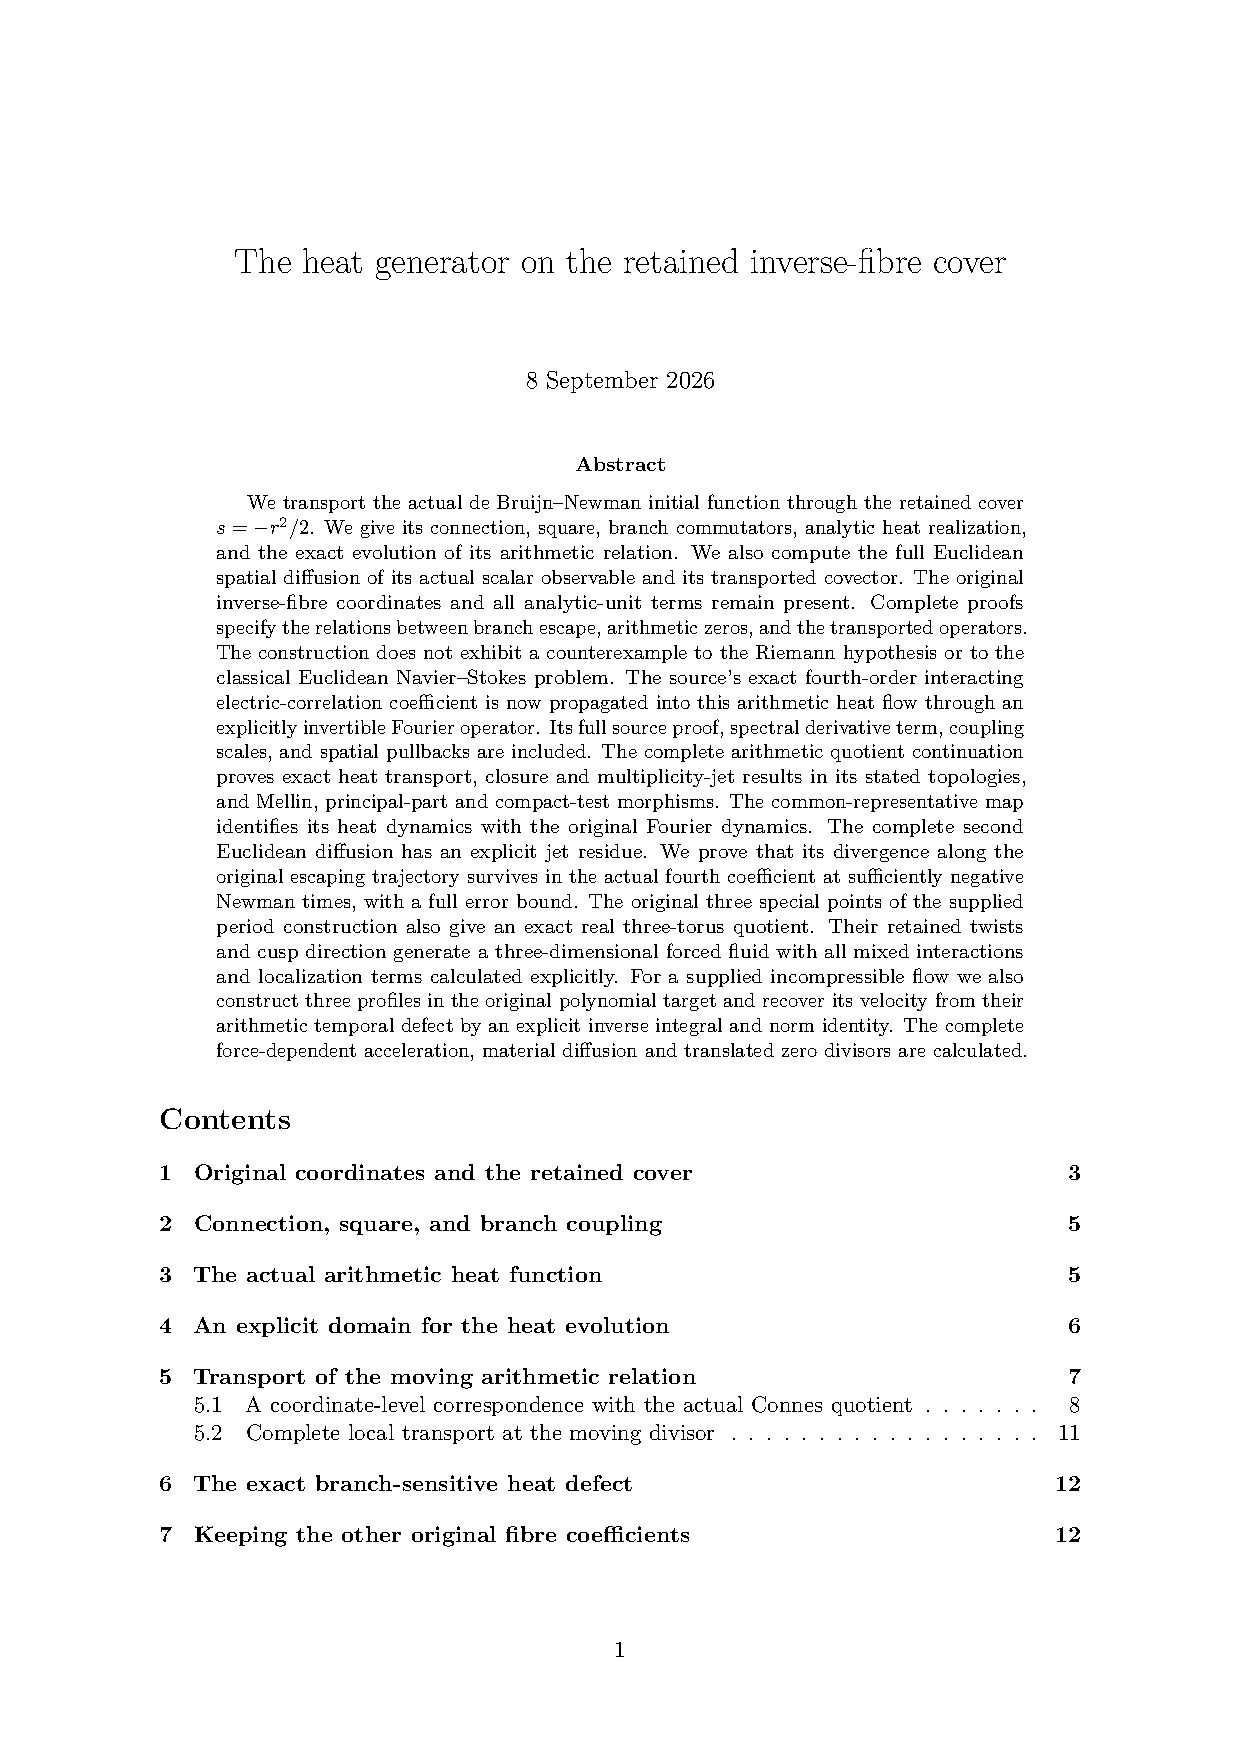
\includepdf[pages=-,addtotoc={1,section,1,{Heat transport on the retained inverse-fibre cover},sidebar-heat}]{sidebar/heat/reader.pdf}
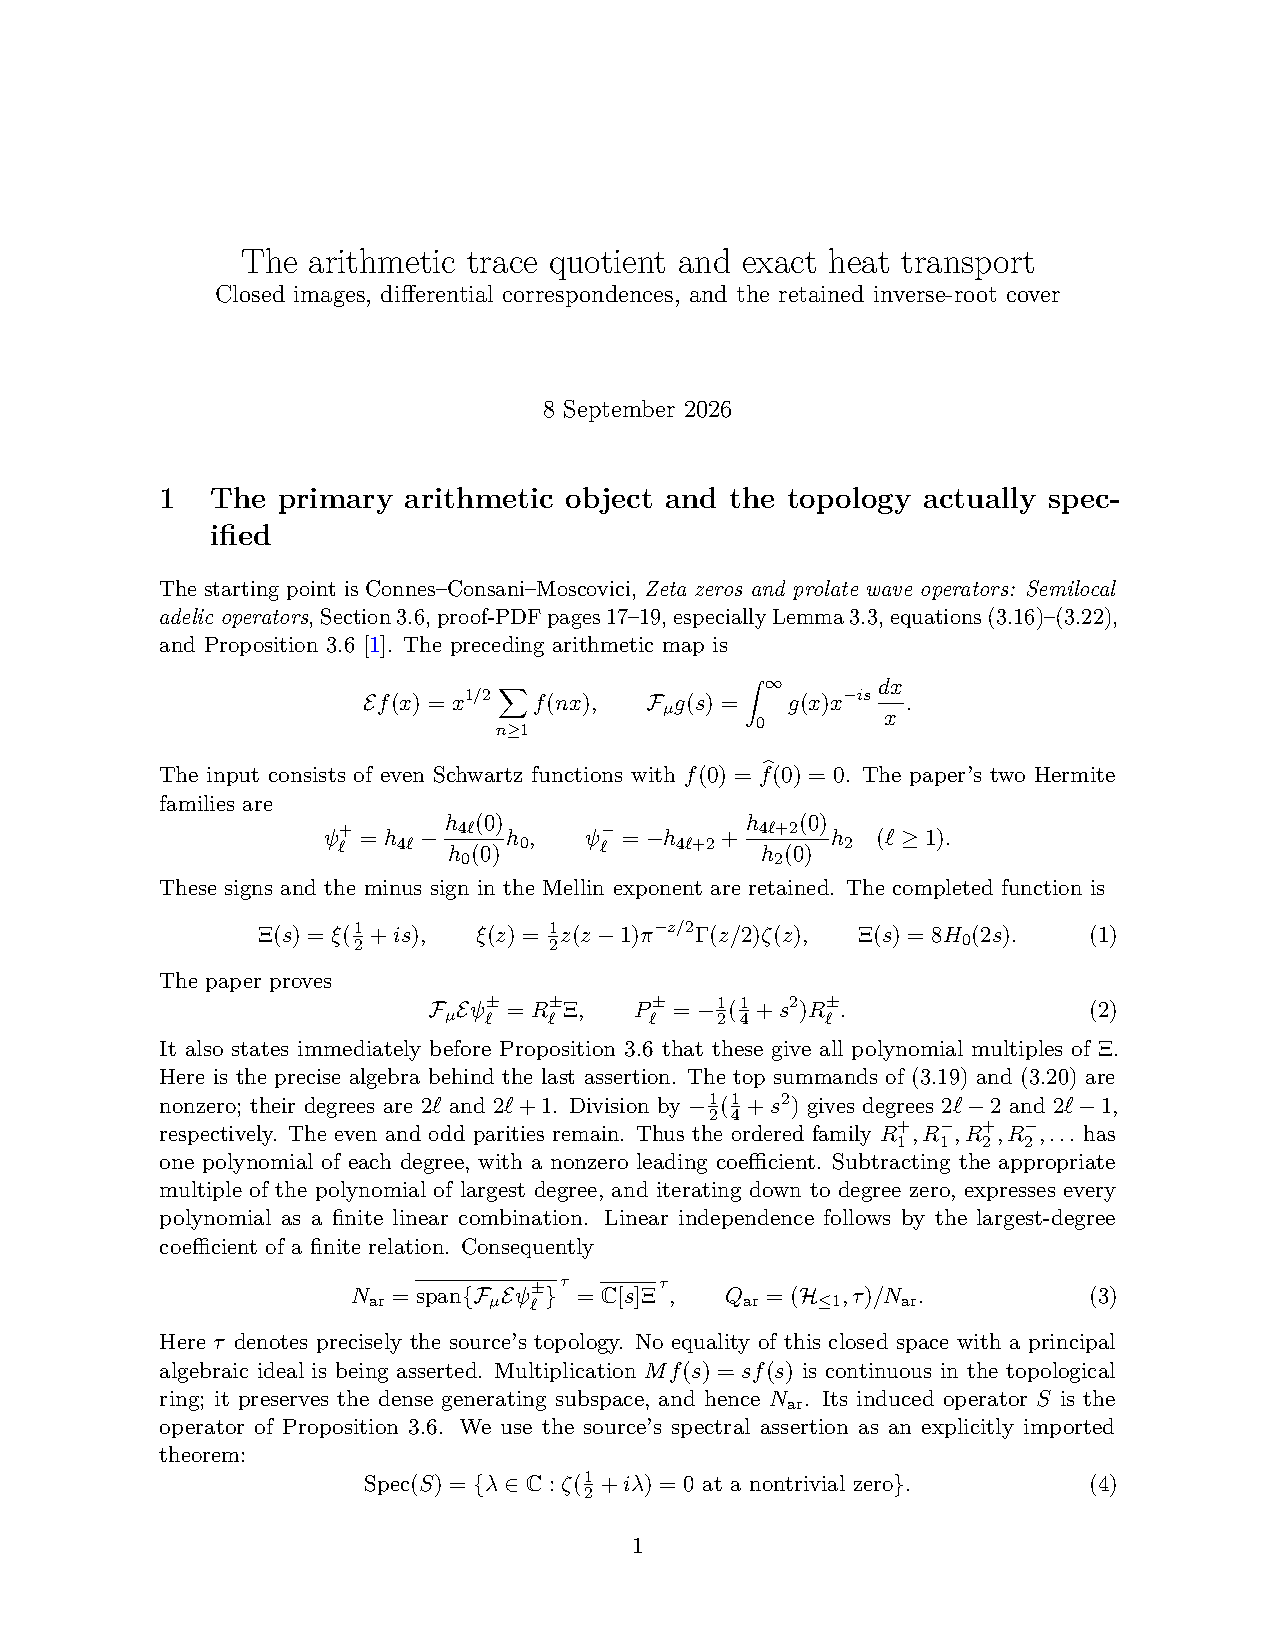
\includepdf[pages=-,addtotoc={1,section,1,{Arithmetic trace quotient and exact heat transport},sidebar-connes}]{sidebar/connes/reader.pdf}
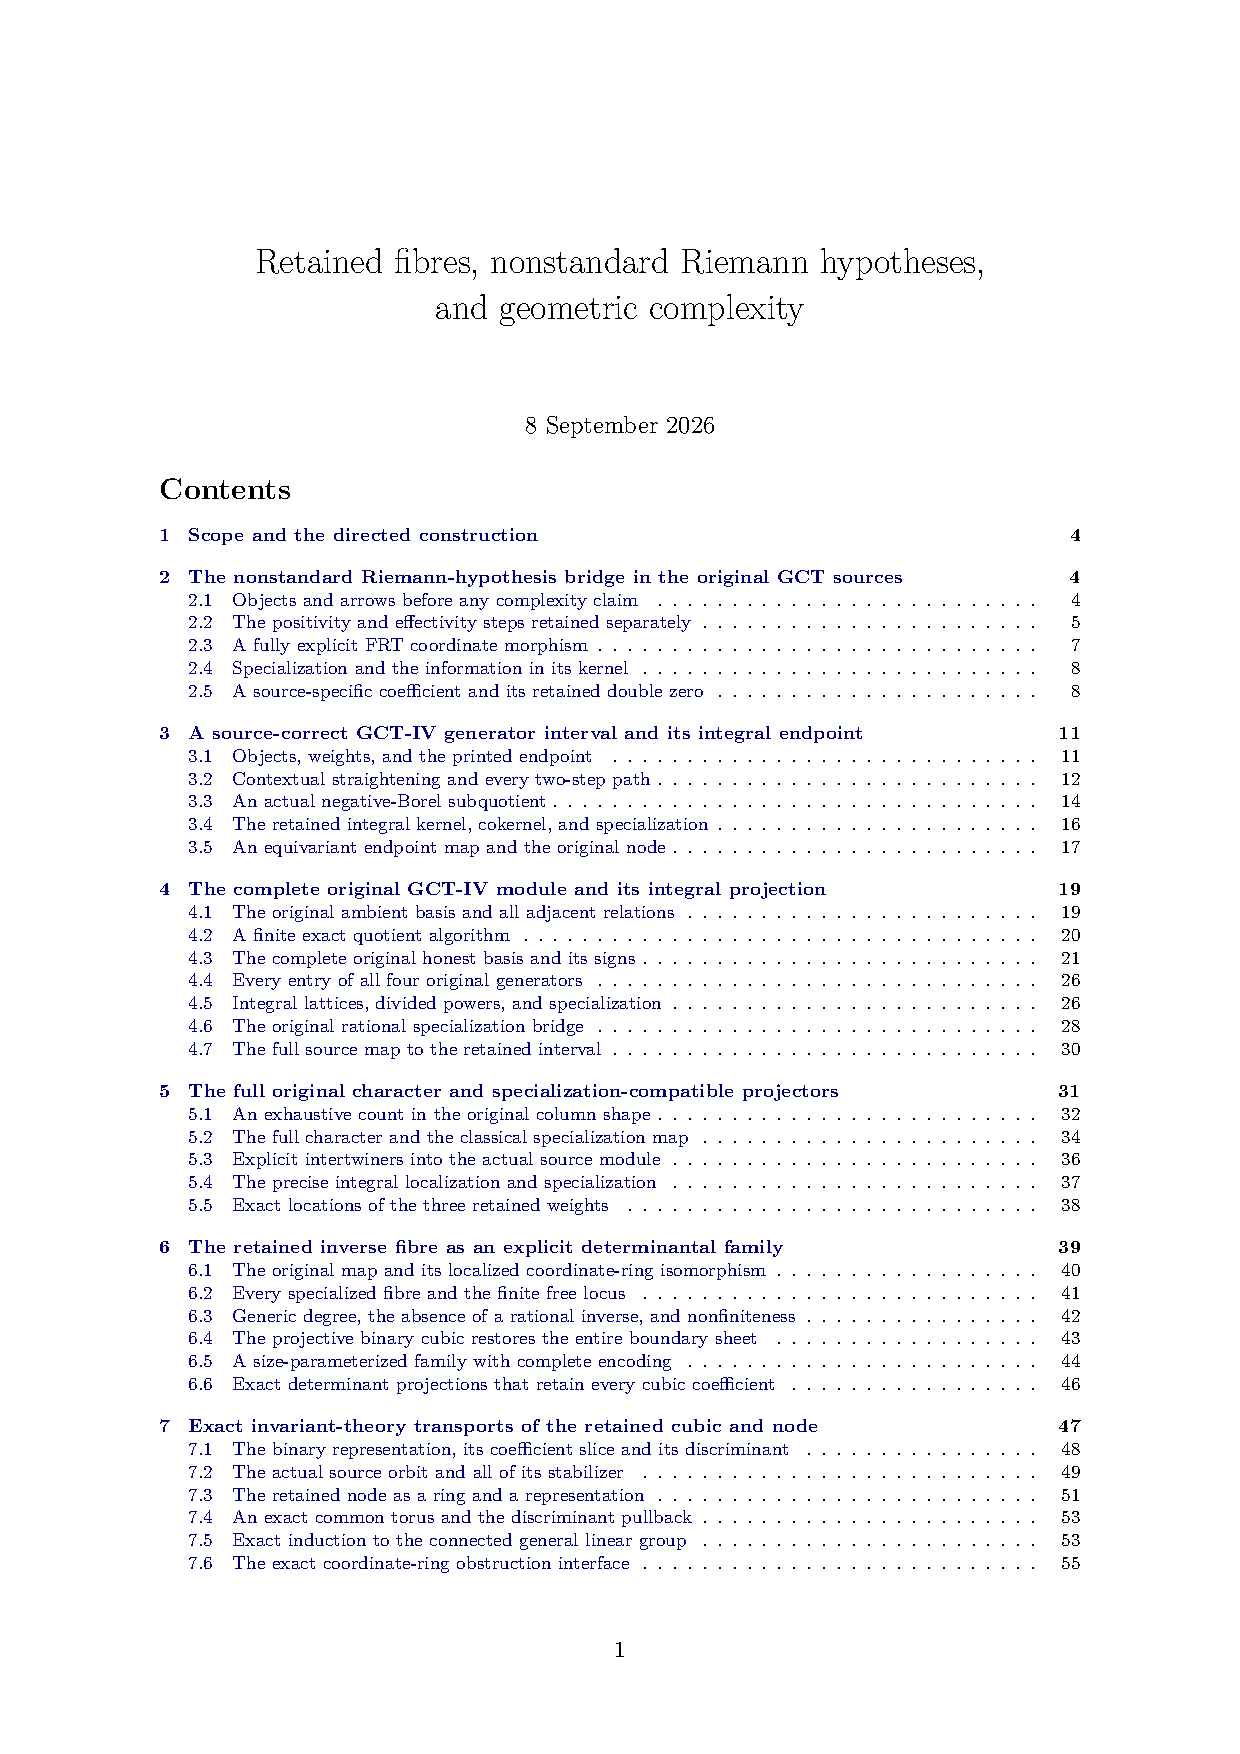
\includepdf[pages=-,addtotoc={1,section,1,{Retained fibres, nonstandard Riemann hypotheses, and geometric complexity},sidebar-gct}]{sidebar/gct/reader.pdf}
\end{document}
